\documentclass[a4paper]{article}

\usepackage{multirow}

\usepackage{tabularx}

\usepackage{graphicx}

\usepackage{multicol}

\usepackage{enumitem}%предостовляет много вариков списка

\usepackage[english, russian]{babel}

\usepackage{hyperref}


\usepackage[%
left=0.50in,%
right=0.50in,%
top=0.8in,%
bottom=1.0in,%
left=0.50in,%
paperheight=11in,%
paperwidth=8.5in,%
]{geometry}%

\setcounter{page}{75}%добовляет нумерацию страниц

\renewcommand*\labelenumi{[\theenumi]}


\begin{document}
\begin{multicols}{2}

\textit{HP ProBook Hewlett Packard} laptop with a \textit{Intel(R)
Core(TM) i7-4900MQ} processor (4 cores with 2 threads)
with a configured core frequency of 3.20 GHz, 16 GB
RAM, and 256 GB SSD. 

At the same time, parallel execution of a small number
of operations over sc-memory (for example, 100 or
10,000 operations) in some cases can be worse than their
sequential execution (Table 2). 

This behavior is related to the peculiarities of the con-
trol mechanisms of the processes in the shared semantic
memory, the classes of operations to be performed, and
their specified input values in the context of the problem
to be solved. For example, all sc-construction search oper-
ations with the same sc-elements, executed in parallel, do
not block each other. For example, the speed of parallel
execution of operations on ostis-system files depends
on the size of the buffer used when reading external
information constructions and writing them to disk, as
well as on the length of the information constructions
themselves.

\begin{tabularx} {0.5\textwidth} {|p{2,5cm}| p{1,5cm}| p{1,5cm}| p{1,5cm}|}
    \cline{1-4}
 \multirow { 2 }{ 2,5cm }{ Number of physical threads } & 1 thread & \multicolumn { 2 }{ |c| }{ 4 thread }  \\ 
\cline{2-4}
& Response time, ms & Response time, ms & Speedup, timestimes\\
\cline{1-4}
\multicolumn { 4 }{|c|}{ Operations addition (modification)} \\  
\cline{1-4}
Operation of scnode creation & 0.099 & 1.306 & 0.076 \\
\cline{1-4}
Operation of scconnector creation & 0.150 & 0.422 & 0.356 \\
\cline{1-4}
Operation of adding content to ostis-system file & 9.521 & 4.128 & 2.307 \\
\cline{1-4}
\multicolumn { 4 }{ |c| }{ Operations of search} \\ 
\cline{1-4}
 Operation of searching sc-connectors outgoing from a given sc-element & 0.530 & 0.241 & 2.200\\
\cline{1-4}
Operation of searching an ostis-system file by its contents & 0.339 & 1.453 & 0.233\\
\cline{1-4}
\multicolumn { 4 }{ |c| }{ Operations of deletion} \\ 
\cline{1-4} 
Operation of deleting an sc-element& 0.144 & 1.494 & 0.096\\
\cline{1-4}
Operation of deleting sc-connectors outgoing from a given sc- element & 0.182 & 0.938 & 0.194\\
\cline{1-4}
 \end{tabularx}





The figure 1 shows Dependence of speedup coefficient
from parallel execution of a group of operations of the
same class on 4 processes on the number of operations
in this group, and the figure 2 shows Dependence of the
execution time of a group of operations on the number
of processes used.\\
\begin{description}
    \item [\textnormal{\textit{C. Efficiency of network operations over sc-memory}}]
\end{description} \par
Network access to sc-memory is provided by the
server subsystem of the ostis-systems software platform,
implemented on the basis of Websocket and JSON
languages (protocols) and providing network operations
(commands) over sc-memory [3].\\
In the process of testing the implementation, the
throughput of its commands was calculated. During the
load testing a test client system implemented in C++ was
used. The same device was used as the device used for
testing operations over sc-memory. As a result, it was
found out that when sending 1000 different commands:
commands for creating sc-elements, commands for pro-
cessing contents of ostis-system files and commands for
deleting sc-elements — the time spent on their processing
did not exceed 0.2 seconds. At the same time, in some
cases it took no more than 0.14 seconds to process 1000
commands for creating sc-elements, while for commands
for deleting sc-elements it took no more than 0.12
seconds, commands for processing the contents of ostis-
system files — no more than 0.10 seconds, commands
to search for sc-constructions isomorphic to a given five-
element graph-template — no more than 0.45 seconds.\\
    \begin{description}
       \item[\textnormal{\textit{D. Conclusions}}]
    \end{description} \par
From the test results, it is clear that the current
implementation of the ostis-systems software platform is
an effective means of processing distributed information
using both the software interface and the network inter-
face and communication protocols.

 The current \textit{Implementation of sc-memory} provides:
 
\begin{itemize}

\item stability in single-threaded and multi-threaded
modes;
\item dast speed of work in single-threaded and multi-
threaded modes;
\item reliability of knowledge and data storage and pro-
cessing in single- and multi-threaded modes.
\end{itemize}

The proposed shared semantic memory model enables
efficient tracking and synchronization of parallel data
accesses. The implementation of this model demonstrates
a significant increase (by 2-3 orders of magnitude) in
the throughput of parallel task execution compared to
previous versions of the platform. However, to ensure
(causal, sequential) consistency of processes and their
operations, besides the data level, it is necessary to
manage the knowledge level [37] .
    \begin{center}
        \appendix V. Conclusion
    \end{center} 

In this paper, a model and implementation of the
shared semantic memory has been proposed and dis-
cussed in detail, including (!):




    \begin{figure*}
        
        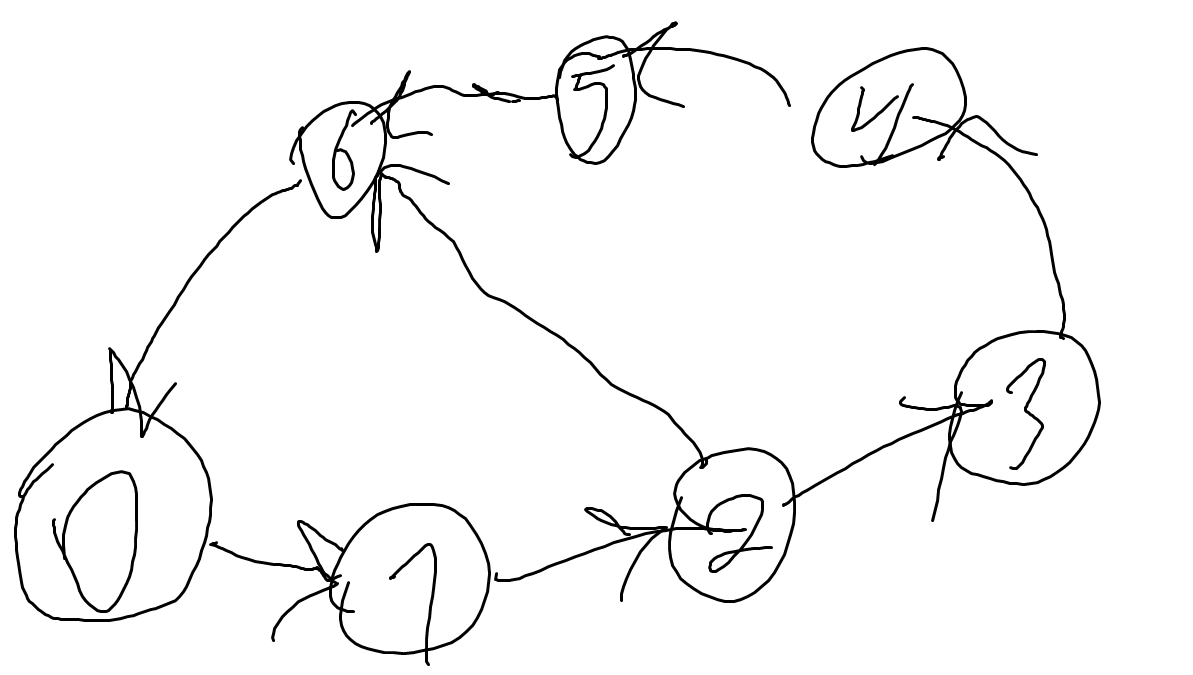
\includegraphics[width=\linewidth]{1.jpg}
        \caption{Dependence of speedup coefficient from parallel execution of a group of operations of the same class on 4 processes on the number of operations in this group}
        
    \end{figure*}

    \begin{figure*}
        
        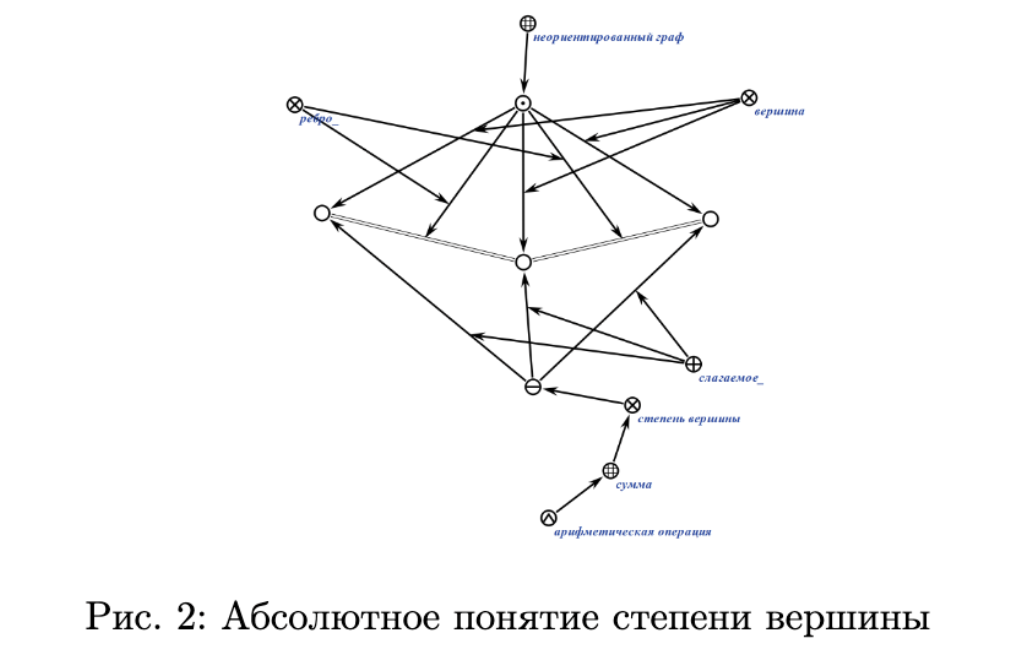
\includegraphics[width=\linewidth]{2.jpg}
        \caption{Dependence of the execution time of a group of operations on the number of processes used}
        
    \end{figure*}


\begin{itemize}
    \item  a storage for unified representation and processing
of graph constructions;
\item a storage for unified representation of string con-
structions used as file contents in graph construc-
tions;
\item a storage for managing events in this memory;
\item a storage for managing processes running in this
memory;
\item a set of operations for working with this memory.
\end{itemize}
The proposed model of the shared semantic memory
includes:
\begin{itemize}
    \item models and algorithms for allocating and releasing
cells in this memory, providing:
    \begin{itemize}
        \item reusability of the released memory segments;
        \item ability to utilize new vacant memory segments;
    \end{itemize}
    \item Models and algorithms to efficiently allocate pro-
cesses in this memory;
    \begin{itemize}
        \item rapid parallel creation of elements in the memory
by allocating processes over the segments of the
memory;
        \item fast unblockable parallel search of constructions,
provided there are no other operations on these
constructions.
    \end{itemize}
    \item Models and algorithms for managing subscriptions
to events in this memory;
    \item Models and algorithms for synchronizing the exe-
cution of processes in the shared memory sections,
providing:
    \begin{itemize}
        \item parallel access to sc-memory, i.e. possibility of parallel execution of actions in sc memory with-out violating correctness of the data structures in it;
        \item absence of deadlocks, races and hungry processes operating in sc-memory.
    \end{itemize}
\end{itemize}
Promising directions to further this line of work are:
\begin{itemize}
    \item development of a model for distributed unified rep-
resentation and processing of information in the
unified semantic memory;
    \item development of a model for representation and stor-
age of platform-dependent agent programs;
    \item development of a consistency model to ensure cor-
rectness of agents’ operation on constructions in the
memory;
    \item development of a model of memory configuration
from the memory itself.
\end{itemize}
In addition, other equally important areas of work are:
\begin{itemize}
    \item improving the documentation of the current Imple-
mentation of sc-memory and the current Software
implementation of ostis-platform;
    \item improvement of methodologies and tools for devel-
oping documentation of software systems;
    \item improvement and mass distribution of the Software
implementation of ostis-platform and intelligent sys-
tems developed on its basis.
\end{itemize}



The formally described model of semantic memory
is consistent with the previously described ontological
model of this memory [3]. The author of this paper
believes that the used approach to modeling of complex
objects will help to simplify the understanding of the
operation of intelligent systems developed according to
the principles of the OSTIS Technology.
    \begin{center}
        \appendix Acknowledgment
    \end{center}


The author would like to thank the scientific teams of
the departments of Intelligent Information Technologies
of Belarusian State University of Informatics and Radio-
electronics and Brest State Technical University for their
help in the work and valuable comments.
    \begin{center}
        \appendix References
    \end{center}
\
\begin{enumerate}
    \item N. Zotov, “Design principles, structure, and development
prospects of the software platform of ostis-systems,” Otkrytye se-
manticheskie tekhnologii proektirovaniya intellektual’nykh system
[Open semantic technologies for intelligent systems], pp. 67—-76,
2023.
\item ——, “Implementation of information retrieval subsystem in
the software platform of ostis-systems,” Otkrytye semanticheskie
tekhnologii proektirovaniya intellektual’nykh system [Open se-
mantic technologies for intelligent systems], pp. 77–94, 2023.
\item ——, “Software platform for next-generation intelligent computer
systems,” in Otkrytye semanticheskie tekhnologii proektirovaniya
intellektual’nykh system [Open semantic technologies for intelli-
gent systems]. BSUIR, Minsk, 2022, pp. 297—-326.
\item V. Golenkov, N. Guliakina, and D. Shunkevich, Otkrytaja
tehnologija ontologicheskogo proektirovanija, proizvodstva
i jekspluatacii semanticheski sovmestimyh gibridnyh
intellektual’nyh komp’juternyh sistem [Open technology of
ontological design, production and operation of semantically
compatible hybrid intelligent computer systems], V. Golenkov,
Ed. Minsk: Bestprint [Bestprint], 2021.

\item V. Golenkov et al., “Associative semantic computers for intelligent
computer systems of a new generation,” in Otkrytye semantich-
eskie tekhnologii proektirovaniya intellektual’nykh system [Open
Semantic Technologies for Intelligent Systems (OSTIS)], vol. 7.
BSUIR, Minsk, 2023, pp. 39–60.

\item V. Golenkov, “Ontology-based design of intelligent systems,”
Otkrytye semanticheskie tekhnologii proektirovaniya intellek-
tual’nykh system [Open semantic technologies for intelligent
systems], pp. 37–56, 2017.

\item D. Shunkevich, “Ontology-based design of hybrid problem
solvers,” in Otkrytye semanticheskie tekhnologii proektirovaniya
intellektual’nykh system [Open semantic technologies for intelli-
gent systems]. Cham: Springer International Publishing, 2022,
pp. 101–131.

\item S. Auer, V. Kovtun, M. Prinz, A. Kasprzik, M. Stocker, and M. E.
Vidal, “Towards a knowledge graph for science,” in Proceedings
of the 8th international conference on web intelligence, mining
and semantics, 2018, pp. 1–6.

\item V. Golenkov, Ed., Tehnologija kompleksnoj podderzhki
zhiznennogo cikla semanticheski sovmestimyh intellektual’nyh
komp’juternyh sistem novogo pokolenija [Technology of complex
life cycle support of semantically compatible intelligent computer
systems of new generation ]. Bestprint, 2023.

\item A. Palagin and N. Petrenko, “To the question of system-
ontological integration of subject area knowledge,” Mathematical
Machines and Systems, vol. 1, no. 3-4, pp. 63–75, 2007.

\item M. Orlov, “Comprehensive library of reusable semantically com-
patible components of next-generation intelligent computer sys-
tems,” in Otkrytye semanticheskie tekhnologii proektirovaniya in-
tellektual’nykh system [Open semantic technologies for intelligent
systems]. Minsk : BSUIR, 2022, pp. 261–272.
\end{enumerate}



\end{multicols}
\end{document}









